\section{Results}
\label{sec:results}

\subsection{Reference Trajectory Example}
\label{sec:reference_trajectory}

To illustrate the end-to-end planning result with one concrete and reproducible case,
we generated a reference request from vertiport `WOHL' to vertiport `KWRD' with a
specified takeoff time of 2026-03-29 06:15:00 UTC and the nominal cruise layer fixed
at \SI{200}{m} MSL. For this request, the A* planner selects the corridor sequence
\[
\texttt{WOHL} \rightarrow \texttt{HAM} \rightarrow \texttt{HOHE} \rightarrow
\texttt{HSEN} \rightarrow \texttt{HCTY} \rightarrow \texttt{TTNB} \rightarrow
\texttt{KWRD},
\]
which the waypoint synthesizer then transforms into a phase-structured trajectory with
departure climb, cruise, and arrival descent segments.

Figure~\ref{fig:reference_trajectory} shows the resulting reference trajectory both in
the horizontal plane and as an altitude-time profile. The synthesized terminal
procedure first climbs vertically from the departure pad and then transitions through
the lower terminal heights before reaching the fixed cruise layer. Along the en-route
portion, the trajectory follows the selected corridor nodes at constant cruise
altitude. Near the destination, the process is reversed through a structured descent
into the arrival pad. The resulting dense 4D trajectory spans approximately
\SI{40.6}{km} and reaches the destination at about 06:46:56 UTC, corresponding to a
flight time of roughly \SI{31.9}{min}.

\begin{figure}[htbp]
  \centering
  \begin{subfigure}[t]{0.49\linewidth}
    \centering
    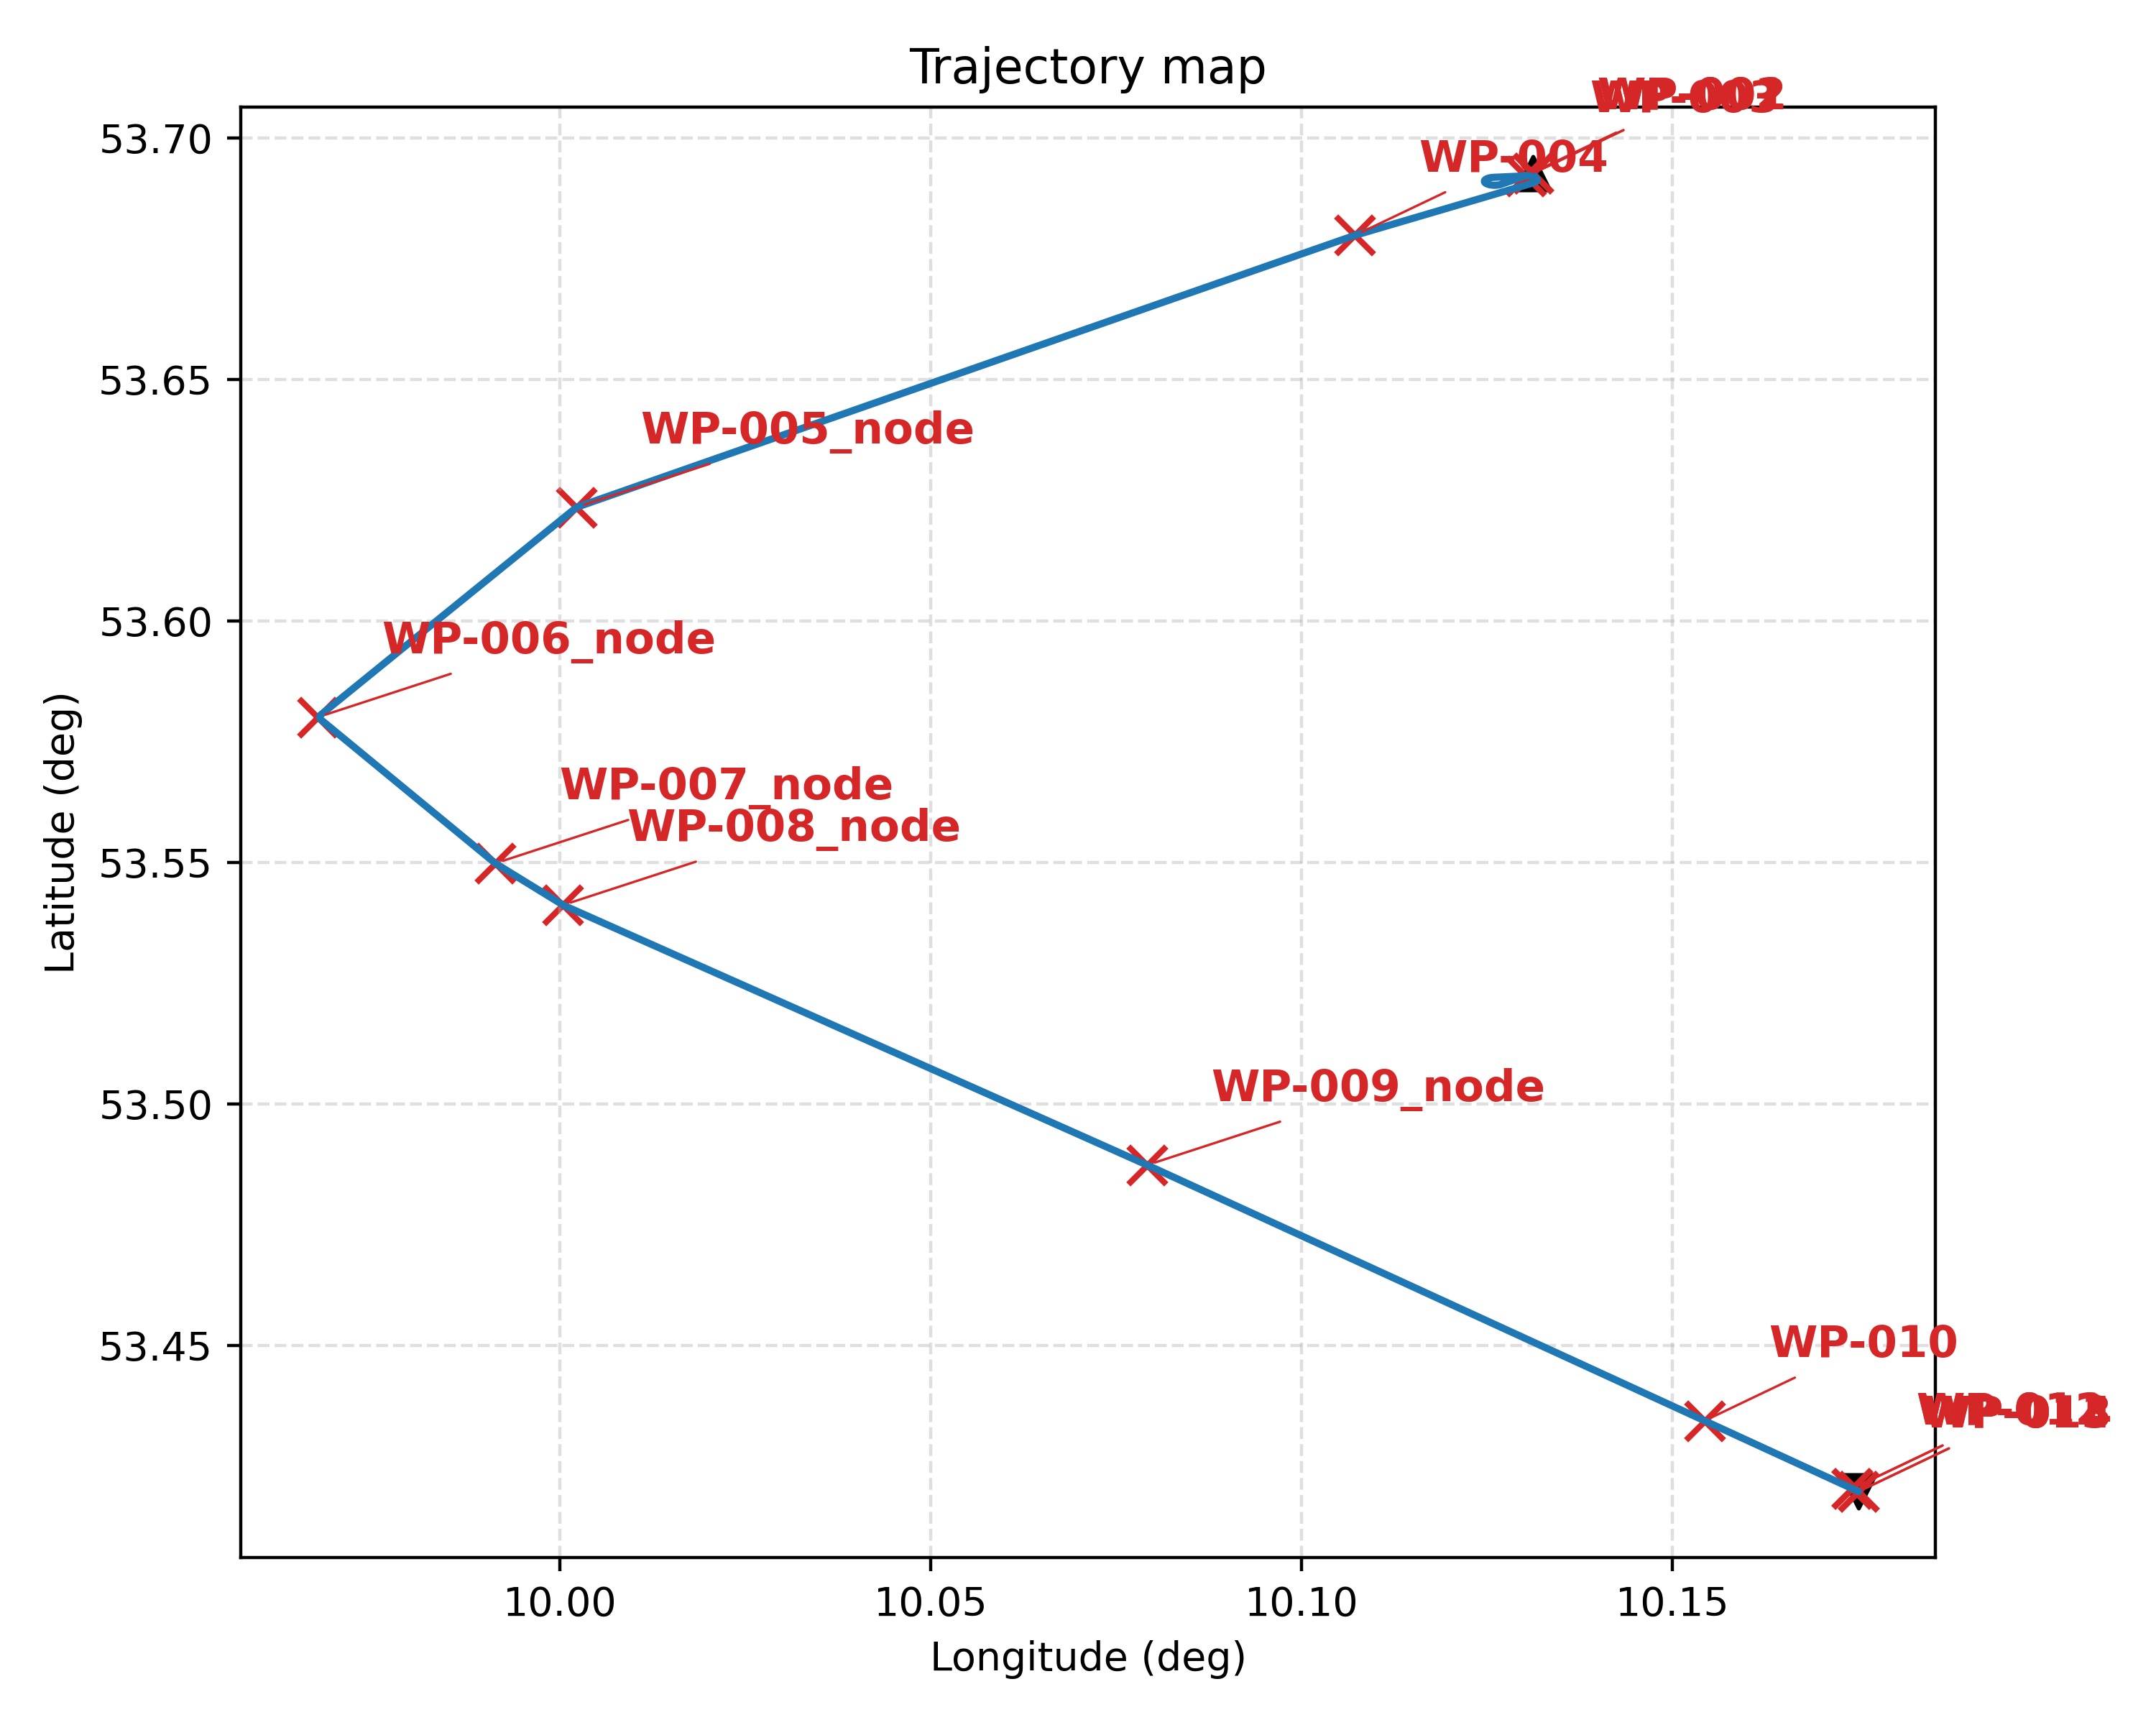
\includegraphics[width=\linewidth]{figures/reference_trajectory_map.png}
  \end{subfigure}
  \hfill
  \begin{subfigure}[t]{0.49\linewidth}
    \centering
    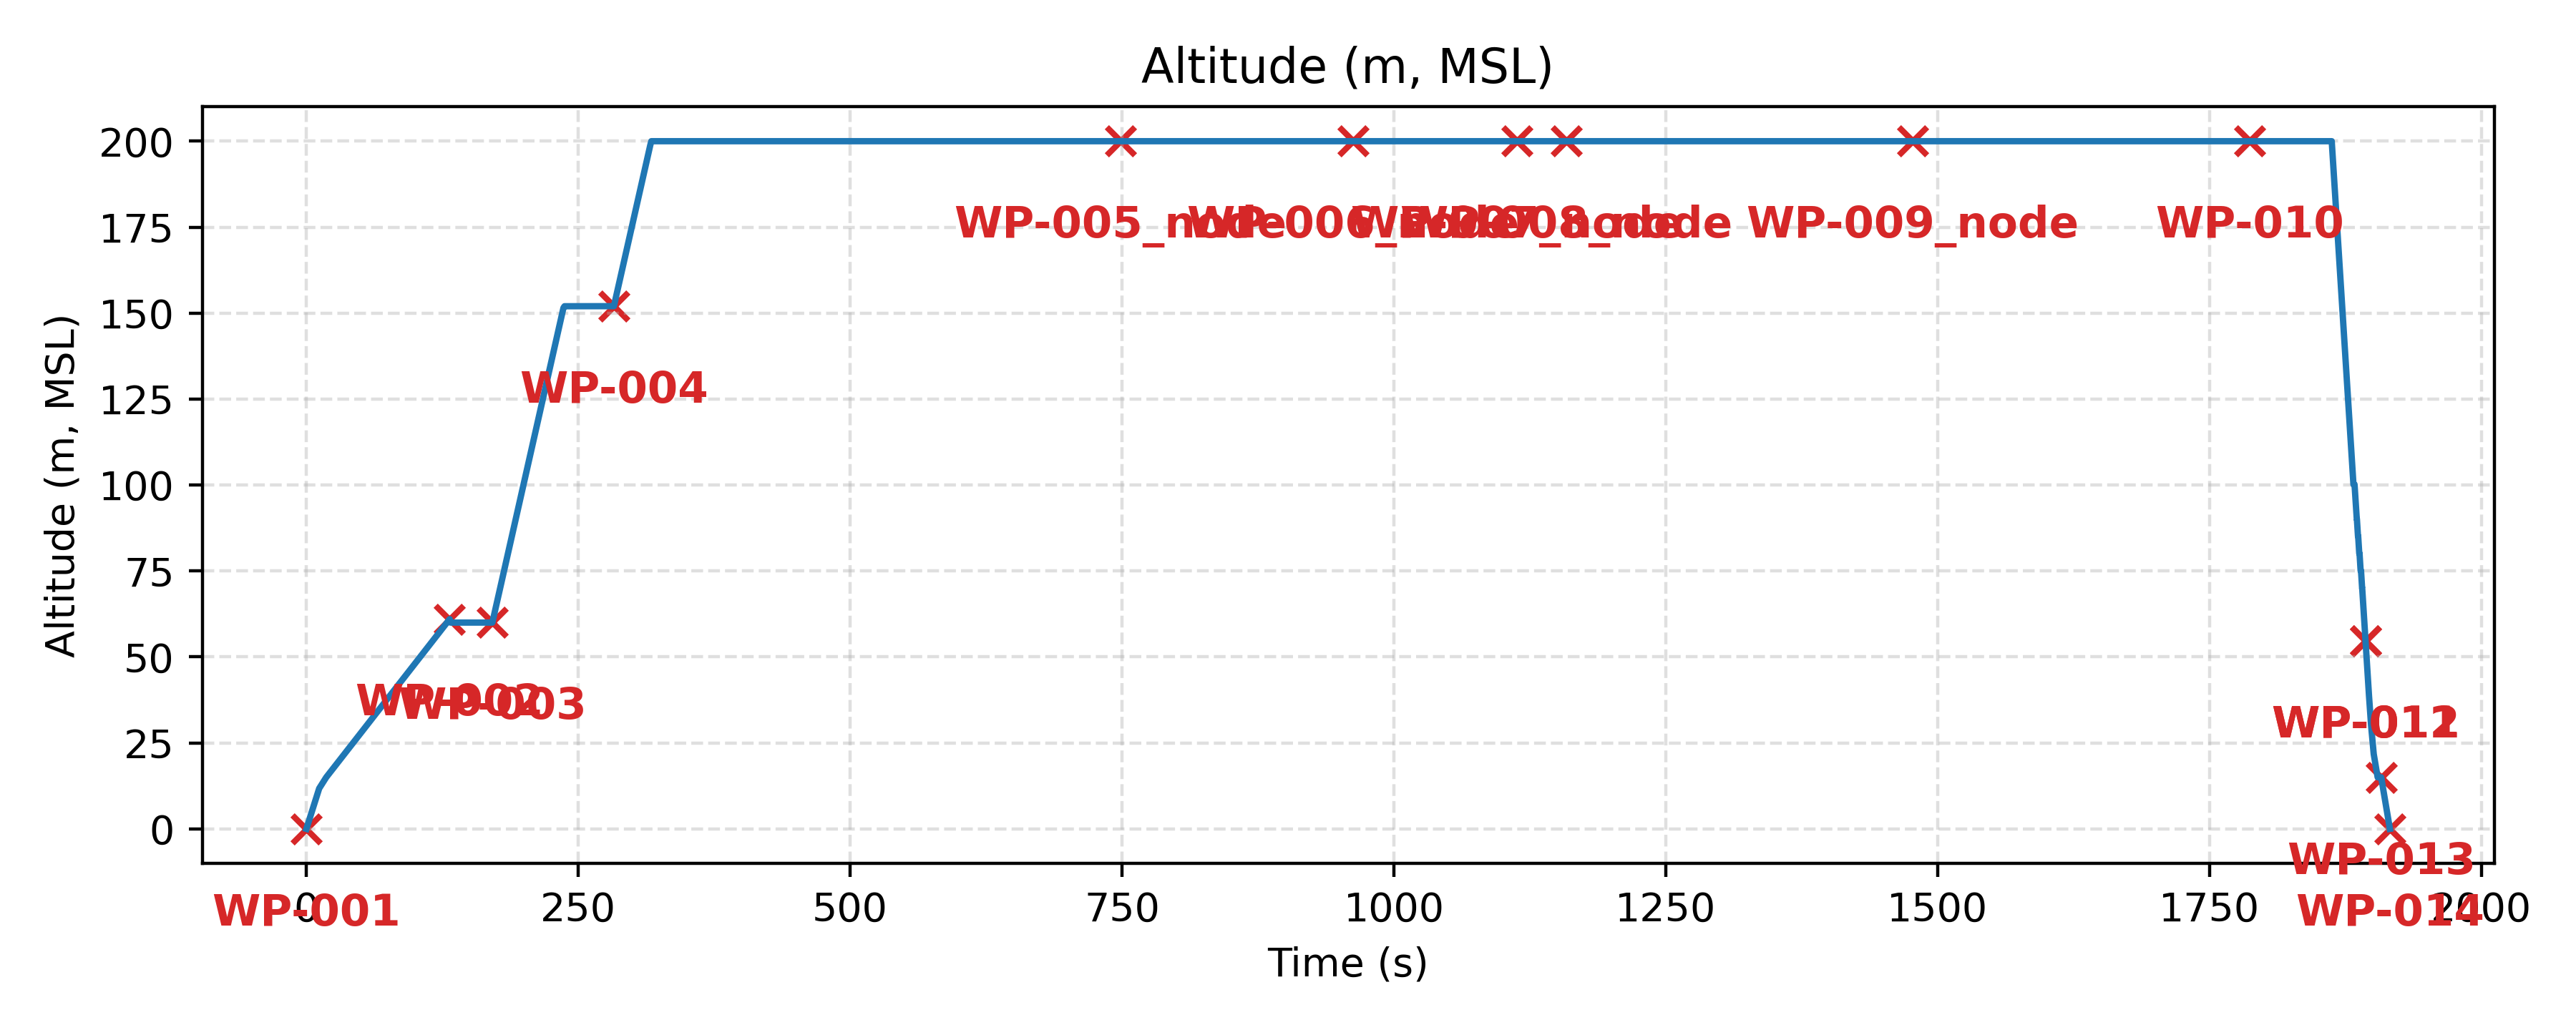
\includegraphics[width=\linewidth]{figures/reference_trajectory_altitude.png}
  \end{subfigure}
  \caption{Reference planning result for the reproducible request
  \texttt{WOHL} to \texttt{KWRD}
  at 2026-03-29 06:15:00 UTC. The left panel shows the lateral path generated from the
  A*-selected corridor sequence, while the right panel shows the corresponding
  altitude-time evolution with climb to the fixed \SI{200}{m} cruise layer and
  structured descent into the destination vertiport. Red markers indicate synthesized
  waypoints used as CFMS inputs.}
  \label{fig:reference_trajectory}
\end{figure}
